\input{myblankpreamble.tex}

\begin{document}

THIS DOC SHOULD NOT HAVE HEADER AND FOOTER, NO TITLE.

How many ways are there to tile a 2-by-12 rectangular region completely 
with 2-by-1 tiles?

Let $a_n$ be the number of ways to put 2-by-1 tiles in a 2-by-$n$
rectangular region.
Tiling left-to-right, the leftmost part of the 2-by-$n$ region
can be tiled by either 
\begin{enumerate}
\item a vertical 2-by-1 tile with a remaining 2-by-$(n-1)$ to be 
tiled, 
\begin{center}
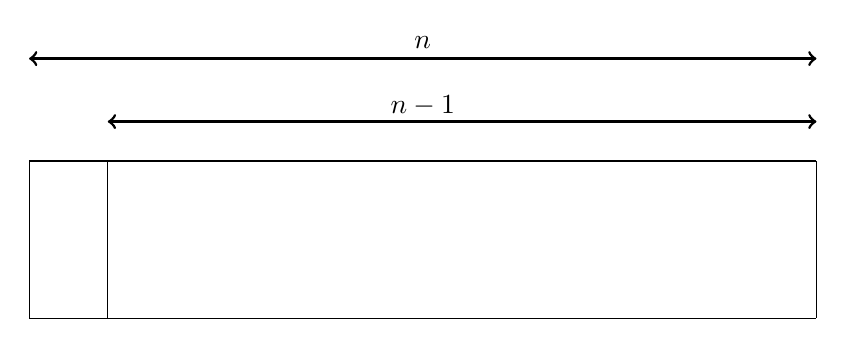
\begin{tikzpicture}

\draw[<->, line width=1pt] (0,1.3) -- (10,1.3);
\node [] at (5, 1.5) {$n$};
\draw[<->, line width=1pt] (1,0.5) -- (10,0.5);
\node [] at (5, 0.7) {$n-1$};
\draw (0,0) -- (10,0);
\draw (0,0) -- (0,-2);
\draw (0,-2) -- (10,-2);
\draw (10,0) -- (10,-2);
\draw (1,0) -- (1,-2);
\end{tikzpicture}
\end{center}
or 
\item two horizontal 1-by-2 tiles with a remaining 2-by-$(n-2)$ region to tile.
\begin{center}
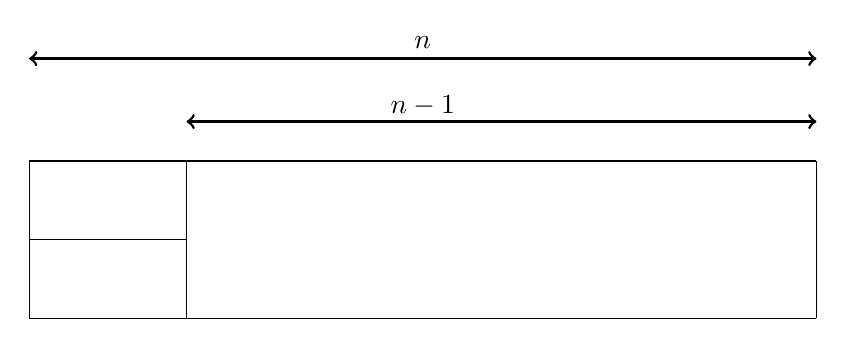
\begin{tikzpicture}
\draw[<->, line width=1pt] (0,1.3) -- (10,1.3);
\node [] at (5, 1.5) {$n$};
\draw[<->, line width=1pt] (2,0.5) -- (10,0.5);
\node [] at (5, 0.7) {$n-1$};
\draw (0,0) -- (10,0);
\draw (0,0) -- (0,-2);
\draw (0,-2) -- (10,-2);
\draw (10,0) -- (10,-2);
\draw (0,-1) -- (2,-1);
\draw (2,0) -- (2,-2);
\end{tikzpicture}
\end{center}
\end{enumerate} 

Therefore
\[
a_n = a_{n-1}+ a_{n-2} \tag{1}
\] 
for $n \geq 2$.
Furthermore $a_1 = 1$ and $a_2 = 2$.
Using (1), we obtain $a_{12} = 233$.

(Using (1), we see that $a_0 = 1$.
and therefore the sequence $a_0, a_1, ...$ 
is the standard Fibonacci sequence.)

\end{document}
